\section{Changing the coefficient boundary and specializing prices}
\label{feedback:sec}

The corner law compares the price of an invertible matrix with that
of an invertible submatrix. We now consider a different operation on
the cell from the preceding section. Write
\[
 K=\begin{pmatrix}M&C\\B&D\end{pmatrix}\in\GL_{n+r}(\C),\qquad
 K(x,w)=(y,w'),\qquad M\in\GL_n(\C).
\]
Closing its state connection at a scalar $s$ means imposing $w=sw'$.
When $I_r-sD$ is invertible, the state equation gives
\[
 w=s(I_r-sD)^{-1}Bx,\qquad
 y=H(s)x,\qquad H(z)=M+zC(I_r-zD)^{-1}B.
\]
Our first objective is to prove $p(H(s))\le p(K)$ whenever $H(s)$
is invertible. We will then prove that a uniform
price bound for a rational matrix at generic scalar values remains
valid at every regular invertible value. Closing the connection serves
only to define the finite matrix $H(s)$; every price inequality concerns
ordinary invertible matrices.

Both arguments use a common comparison between coefficient boundary
conditions. The data-to-data block of the preceding cascade is multiplication
by a matrix series modulo $z^t$. We compare this with multiplication
modulo a different scalar polynomial of degree $t$. For a $k$th tensor
power, a scalar change of coordinates confines the discrepancy to
$O(k)$ time indices. We must also control the large spatial matrix on
those indices: an explicit common family of inexpensive generators
supplies this second bound. The resulting estimate is uniform over the
scalar modulus, which can therefore be chosen separately at each tensor
order.

We retain the time coefficient convention for $\mathcal T_t$: for a
matrix series $F(z)$ regular at zero, $\mathcal T_t(F)$ sends the
coefficients of $x(z)$, of degree less than $t$, to those of $F(z)x(z)$
modulo $z^t$, with the time index outermost. All prices in this section
satisfy the laws of \cref{thm:prices}.

\subsection{A uniform comparison for scalar moduli}

\begin{lemma}[Coefficient-boundary comparison]
\label{lem:boundary-comparison}
Fix $G(z)\in\Mat_n(\C[z])$ with $G(0)$ invertible.  There is a constant
$C_G$ with the following property.  Let $k\geq1$, put $N=n^k$ and
$d=k\deg G$, and let $t>d$ be an integer.  Suppose $\ell(z)$ is monic of
degree $t$, $\ell(0)\ne0$, and multiplication by $G(z)^{\otimes k}$ on
$(\C[z]/(\ell))^N$ is invertible.  Denote its matrix in the coefficient
basis by $W$, and put
\[
 A_G=\mathcal T_t(G(z)^{\otimes k}).
\]
Then
\begin{equation}
 \bigl|p(W)-p(A_G)\bigr|
 \leq C_G N\bigl(t\log(2t)+(k+1)^6\bigr).
 \label{feedback:eq:boundary-error}
\end{equation}
The constant is independent of $k,t,\ell$ and of the magnitudes of the
coefficients of $\ell$.  In particular, for
\begin{equation}
 t=t(k)=2^{\lceil 8\log_2(k+1)\rceil},
 \qquad (k+1)^8\leq t<2(k+1)^8,
 \label{feedback:eq:common-length}
\end{equation}
the difference is $o(tkN)$, uniformly over every admissible modulus of
that degree.
\end{lemma}

\begin{proof}
Choose once and for all polynomial $J(z)$ and scalar polynomial $u(z)$
such that
\[
 G(z)^{-1}=J(z)/u(z),\qquad u(0)\ne0;
\]
for example, take $J=\operatorname{adj}G$ and $u=\det G$.  Write
\[
 G_k(z)=G(z)^{\otimes k}=\sum_{j=0}^{d}G_jz^j,
 \qquad
 J_k(z)=J(z)^{\otimes k}=\sum_{i=0}^{e}J_iz^i,
 \qquad e=k\deg J.
\]
These are degree bounds with zero coefficient matrices permitted.
The subscript on $G_j$ or $J_i$ in this proof denotes a coefficient of
the tensor power, rather than of the original fixed matrix.
Both $d$ and $e$ are bounded by a fixed multiple of $k$.
If $d=0$, multiplication is coefficientwise, so $W=A_G$ and the result
holds.  Assume $d>0$ and set $T=t-d$.

Let $L=W-A_G$.  An input supported at times less than $T$ has product
with $G_k$ of degree less than $t$, so $L$ has zero columns at those
times.  Scalar polynomial division also shows that, for every input
$x(z)$ of degree less than $t$,
\begin{equation}
 Lx=\ell(z)v_x(z)\pmod {z^t},\qquad \deg v_x<d.
 \label{feedback:eq:boundary-quotient}
\end{equation}
Here $v_x$ is minus the quotient of $G_kx$ by $\ell$, with scalar
division applied to every coordinate.  The degree bound follows from
$\deg(G_kx)<t+d$.

The invertible relative map and the scalar prefix map are
\[
 R=A_G^{-1}W=I+S,\qquad S=A_G^{-1}L,
 \qquad
 P=\mathcal T_T(u^k/\ell)\oplus I_d.
\]
The series in $P$ is regular and nonzero at zero.  Since $S$ has zero
prefix columns and $P^{-1}$ is identity on the suffix of length $d$,
\begin{equation}
 S(P^{-1}\otimes I_N)=S,\qquad
 \widehat R=(P\otimes I_N)R(P^{-1}\otimes I_N)
           =I+(P\otimes I_N)S.
 \label{feedback:eq:prefix-conjugation}
\end{equation}
This identity uses the entire prefix--suffix decomposition; a general
scalar change of basis on all $t$ times would not have this property.

On the prefix, the output of the correction in
\cref{feedback:eq:prefix-conjugation} is, modulo $z^T$,
\[
 \frac{u^k}{\ell}\frac{J_k}{u^k}\ell v_x=J_kv_x.
\]
It therefore vanishes at prefix times greater than or equal to $e+d$.
Define the disjoint sets
\[
 \mathcal E=\{0,\ldots,\min(T,e+d)-1\},\quad
 \mathcal B=\{T,\ldots,t-1\},\quad
 \mathcal U=\mathcal E\cup\mathcal B.
\]
The correction has columns only in $\mathcal B$ and rows only in
$\mathcal U$, where $|\mathcal U|\leq e+2d=O(k)$.
Thus both blocks coupling $\mathcal U$ to its complement are zero in
the correction.  A simultaneous permutation of rows and columns gives
\begin{equation}
 \widehat R\simeq R_{\mathcal U}\oplus
 I_{(t-|\mathcal U|)N},
 \qquad R_{\mathcal U}\in\GL_{|\mathcal U|N}(\C).
 \label{feedback:eq:active-summand}
\end{equation}
Invertibility of the active block follows from invertibility of
$\widehat R$.  If the coarse early and suffix ranges would overlap,
the minimum in $\mathcal E$ truncates the former: the middle set is
then empty and $t\leq e+2d$.  The bound and the direct-sum conclusion
still hold.  \Cref{feedback:fig:boundary-support} displays the support
of the correction $\widehat R-I$ when the middle set is nonempty.

\begin{figure}[t]
\centering
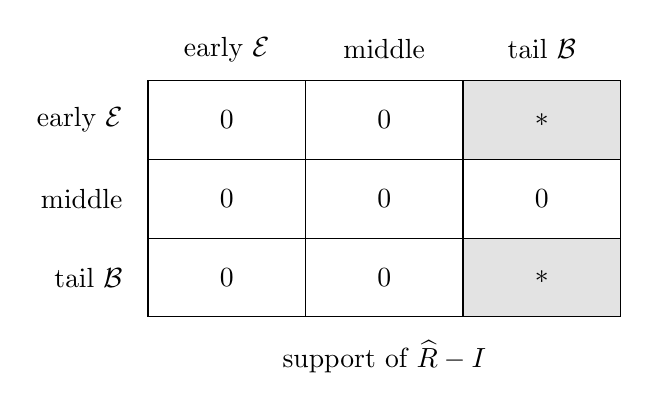
\begin{tikzpicture}[x=1cm,y=1cm]
 \fill[gray!22] (4,2) rectangle (6,3);
 \fill[gray!22] (4,0) rectangle (6,1);
 \draw (0,0) rectangle (6,3);
 \draw (2,0)--(2,3) (4,0)--(4,3);
 \draw (0,1)--(6,1) (0,2)--(6,2);
 \node at (1,3.4) {early $\mathcal E$};
 \node at (3,3.4) {middle};
 \node at (5,3.4) {tail $\mathcal B$};
 \node[anchor=east] at (-.2,2.5) {early $\mathcal E$};
 \node[anchor=east] at (-.2,1.5) {middle};
 \node[anchor=east] at (-.2,.5) {tail $\mathcal B$};
 \foreach \x/\y in {1/.5,1/1.5,1/2.5,3/.5,3/1.5,3/2.5,5/1.5}
   \node at (\x,\y) {$0$};
 \node at (5,2.5) {$*$};
 \node at (5,.5) {$*$};
 \node at (3,-.5) {support of $\widehat R-I$};
\end{tikzpicture}
\caption{After prefix conjugation, only the shaded blocks can be
nonzero in the correction.  Restoring the identity leaves the middle
coordinates as an identity direct summand.  The picture shows the case
with a nonempty middle; the definition of $\mathcal E$ also covers an
empty middle.}
\label{feedback:fig:boundary-support}
\end{figure}

The small number of active times alone would not bound the cost of
their $N\times N$ spatial blocks.  We next give an indexed formula
that controls those blocks uniformly.  For each integer $m\geq0$ that
occurs below, divide the scalar monomial $z^m$ by $\ell$ and write
\[
 z^m=\ell(z)q_m(z)+r_m(z),\qquad \deg r_m<t,
 \qquad q_{s,m}=[z^s]q_m(z).
\]
For $m=b+j$ with $0\leq b<t$ and $0\leq j\leq d$, we have
$\deg q_m<d$.  Set $q_{s,m}=0$ when $s<0$ or $s\geq d$; also
$q_m=0$ when $m<t$.  Let
\[
 \eta_h=[z^h](\ell/u^k),\qquad \eta_h=0\quad(h<0).
\]
All these scalars may depend on $k,t,\ell$.
For $0\leq a,b<t$, define
\begin{equation}
 \gamma_{abij}=
 \begin{cases}
  -q_{a-i,b+j},&a<T,\\[2pt]
  -\displaystyle\sum_{s=0}^{d-1}\eta_{a-i-s}q_{s,b+j},&a\geq T.
 \end{cases}
 \label{feedback:eq:ordered-coefficients}
\end{equation}
Then the exact block formula is
\begin{equation}
 \widehat R_{ab}=\delta_{ab}I_N+
    \sum_{i=0}^{e}\sum_{j=0}^{d}\gamma_{abij}J_iG_j.
 \label{feedback:eq:ordered-span}
\end{equation}
Indeed, on an input $z^bx_b$, scalar division gives
$v_x=-\sum_jq_{b+j}G_jx_b$ in
\cref{feedback:eq:boundary-quotient}.  The prefix correction is $J_kv_x$,
which gives the first case of
\cref{feedback:eq:ordered-coefficients}.  The suffix is unchanged by the
left prefix map, so its correction is $(\ell/u^k)J_kv_x$ modulo $z^t$,
which gives the second case.  Right conjugation has already disappeared
by \cref{feedback:eq:prefix-conjugation}.  Every spatial product is
ordered as $J_iG_j$: no commutation of coefficient matrices is used.
Reduction and scalar convolution introduce only the displayed scalar
weights, irrespective of the length of the underlying coefficient
lists.

Here is a gate count for applying the active block.  Applying a fixed
$n\times n$ matrix on each of the $N/n$ fibers of one tensor axis uses
at most $2nN$ scalar gates, by direct multiplication and addition.
Consequently $G(\xi)^{\otimes k}$ applies in at most $2nkN$ gates for
any $\xi\in\C$, including points where $G(\xi)$ is singular.  At
$d+1$ distinct points, interpolation expresses any chosen coefficient
$G_j$ as a scalar linear combination of these evaluation matrices.
Running the $d+1$ evaluation circuits on the same input and combining
their outputs uses at most
\[
 2nkN(d+1)+2(d+1)N=O_G((k+1)^2N)
\]
gates.  The same argument with $e+1$ points applies to $J_i$, so the
ordered product $J_iG_j$ has a circuit of this order by composition.
No inverse of an evaluation matrix is needed; only the scalar
Vandermonde interpolation matrix is inverted in choosing constants.

There are $O_G((k+1)^2)$ active ordered pairs of time indices and
$(e+1)(d+1)=O_G((k+1)^2)$ spatial generators in
\cref{feedback:eq:ordered-span}.  For each active block entry, apply
each required generator to its input vector, multiply its output by
$\gamma_{abij}$, and add the resulting vectors.  The generator
applications cost $O_G((k+1)^6N)$ gates in total.  The scalar weights
and output additions cost only $O_G((k+1)^4N)$ additional gates, and
the identity contribution uses the already available input values.
The output count is $|\mathcal U|N=O_G((k+1)N)$.  Thus the universal
one-way DAG bound, \cref{cor:dag-price}, and
\cref{feedback:eq:active-summand} give
\begin{equation}
 p(\widehat R)=p(R_{\mathcal U})
        \leq C_G(k+1)^6N.
 \label{feedback:eq:active-cost}
\end{equation}
The potentially complicated coefficients in
\cref{feedback:eq:ordered-coefficients} are prechosen circuit scalars.
Every use of such a scalar has been charged; the model does not charge
for producing its description.  This is precisely why the gate bound
is independent of $t$ and $\ell$.

By \cref{lem:scalar-convolution}, direct-sum additivity and the tensor
law,
\[
 p(P)=O(T\log(2T))=O(t\log(2t)),\qquad
 p(P\otimes I_N)=Np(P).
\]
Undoing the conjugation and using inverse symmetry gives
\[
 p(R)=p(R^{-1})\leq2Np(P)+C_G(k+1)^6N.
\]
Finally $W=A_GR$ and $A_G=WR^{-1}$ imply
$|p(W)-p(A_G)|\leq p(R)$, proving
\cref{feedback:eq:boundary-error}.  Dividing that bound by $tkN$ gives
\begin{equation}
 \frac{|p(W)-p(A_G)|}{tkN}
 \leq C_G\left(\frac{\log(2t)}{k}
           +\frac{(k+1)^6}{tk}\right).
 \label{feedback:eq:normalized-error}
\end{equation}
For the choice of $t$ in \cref{feedback:eq:common-length}, both terms tend to zero.  Also
$t>d$ eventually, since $G$ was fixed before $k$ grows.  Every estimate
holds uniformly for all admissible $\ell$ at that $k,t$.
\end{proof}

\subsection{Closing a state connection}

\begin{samepage}
\begin{theorem}[Feedback law]
\label{thm:feedback}
Let
\[
 K=\begin{pmatrix}M&C\\B&D\end{pmatrix}\in\GL_{n+r}(\C),
 \qquad M\in\GL_n(\C),
 \qquad H(z)=M+zC(I_r-zD)^{-1}B.
\]
If $s_0\in\C$ satisfies
\[
 \det(I_r-s_0D)\ne0,\qquad \det H(s_0)\ne0,
\]
then
\begin{equation}
 p(H(s_0))\leq p(K).
 \label{feedback:eq:feedback-law}
\end{equation}
No invertibility of $D$ is required.
\end{theorem}
\end{samepage}

\begin{proof}
If there is no state block, $H=M=K$.  With a state block present,
$s_0=0$ is the invertible corner law, \cref{thm:corner}.  We prove the
claim for $s_0\ne0$ by fixing $K,s_0$ throughout the following estimates.
Let
\[
 q(z)=\det(I_r-zD),\qquad
 G(z)=q(z)M+zC\operatorname{adj}(I_r-zD)B=q(z)H(z).
\]
Then $G$ is polynomial, $q(0)=1$, $q(s_0)\ne0$ and $G(0)=M$ is
invertible.  Put $N=n^k$ and choose $t=t(k)$ as in
\cref{feedback:eq:common-length}.  For sufficiently large $k$, this
choice meets the degree condition in \cref{lem:boundary-comparison}.

Write $A_H=\mathcal T_t(H(z)^{\otimes k})$.  The cascade estimate in
\cref{corner:eq:cascade-bound} gives, with constants depending only
on the fixed cell,
\begin{equation}
 p(A_H)\leq tk n^{k-1}p(K)
     +C_KN\bigl(t\log(2t)+(k+1)^3\bigr).
 \label{feedback:eq:cascade-use}
\end{equation}
Moreover,
\[
 A_G=(\mathcal T_t(q^k)\otimes I_N)A_H,
\]
and the scalar factor is invertible.  The scalar-convolution bound
and the product law in both directions show that
\begin{equation}
 |p(A_G)-p(A_H)|\leq C N t\log(2t).
 \label{feedback:eq:clear-denominator-cost}
\end{equation}
Its constant is independent of the degree or coefficients of $q^k$.

Apply the coefficient-boundary comparison with
$\ell(z)=(z-s_0)^t$.  To verify its remaining invertibility hypothesis,
translate a polynomial to its coefficients at $s_0$.  The scalar
translation matrix $V_{s_0}$ has entries
\[
 (V_{s_0})_{ij}=
 \begin{cases}\binom ji s_0^{j-i},&j\geq i,\\0,&j<i,
 \end{cases}
 \qquad 0\leq i,j<t.
\]
It is invertible with inverse $V_{-s_0}$.  In the translated
coordinates, multiplication modulo $(z-s_0)^t$ becomes multiplication
by $G(s_0+w)^{\otimes k}$ modulo $w^t$.  Hence
\begin{equation}
 (V_{s_0}\otimes I_N)W(V_{s_0}^{-1}\otimes I_N)
   =\mathcal T_t(G(s_0+w)^{\otimes k}).
 \label{feedback:eq:taylor-conjugacy}
\end{equation}
The right-hand side is lower triangular in time, with repeated
invertible diagonal block $G(s_0)^{\otimes k}$.  Thus $W$ is
invertible, as required.

The price of translation is also small.  If $D_!=\diag(0!,1!,\ldots,
(t-1)!)$ and $U_{s_0}$ is the upper triangular Toeplitz matrix with
entry $s_0^{j-i}/(j-i)!$ at $j\geq i$, then
\[
 V_{s_0}=D_!^{-1}U_{s_0}D_!.
\]
Monomial invariance, transpose symmetry and
\cref{lem:scalar-convolution} imply
\begin{equation}
 p(V_{s_0})=O(t\log(2t)).
 \label{feedback:eq:translation-price}
\end{equation}
Applying triangular monotonicity, \cref{lem:triangular}, to
\cref{feedback:eq:taylor-conjugacy}, then undoing its two scalar
changes of basis, gives
\begin{align}
 p(W)
 &\geq t\,p(G(s_0)^{\otimes k})-2Np(V_{s_0})\notag\\
 &=tk n^{k-1}p(H(s_0))-O(Nt\log(2t)).
 \label{feedback:eq:feedback-lower}
\end{align}
For the equality, use the tensor law and the nonzero scalar relation
$G(s_0)=q(s_0)H(s_0)$, which preserves price.

Combining \cref{feedback:eq:boundary-error,feedback:eq:cascade-use,feedback:eq:clear-denominator-cost,feedback:eq:feedback-lower} yields
\[
 tk n^{k-1}\bigl(p(H(s_0))-p(K)\bigr)
 \leq C_{K,s_0}N\bigl(t\log(2t)+(k+1)^6\bigr).
\]
Divide by $tk n^{k-1}=tkN/n$ and let $k$ tend to infinity with the
single fixed choice of $t$ in \cref{feedback:eq:common-length}.  The error
vanishes by \cref{feedback:eq:normalized-error}, proving
\cref{feedback:eq:feedback-law}.
\end{proof}

\subsection{Specialization at any regular invertible value}

\begin{theorem}[Algebraic specialization]
\label{thm:specialization}
Let $X(z)\in\Mat_n(\C(z))$ be regular at $z_0\in\C$, and assume
$X(z_0)$ is invertible.  Suppose there are a finite set $E\subset\C$
and a real constant $C_0$ such that, for every $s\notin E$, the matrix
$X(s)$ is defined and invertible and
\[
 p(X(s))\leq C_0.
\]
Then $p(X(z_0))\leq C_0$.
\end{theorem}

\begin{proof}
Replace $X(z)$ by $X(z_0+z)$ and $E$ by $E-z_0$, so it suffices to
treat $z_0=0$.  By regularity, the entries have polynomial denominator
representations nonzero at zero.  Their product gives a scalar
polynomial $q$ with $q(0)\ne0$ for which $G=qX$ is polynomial.
In particular $G(0)$ is invertible.  Enlarge the finite exceptional
set to
\[
 E'=E\cup\{s:q(s)=0\}.
\]
At every $s\notin E'$, the matrix $G(s)$ is invertible and
$p(G(s))=p(X(s))\leq C_0$.

Fix $X,q,E'$ before letting $k$ grow, put $N=n^k$, and again choose
the single run length specified in \cref{feedback:eq:common-length}.  For each
such finite $t$, let $\zeta_t$ be the specified primitive $t$th root
of unity.  Choose
\begin{equation}
 a=a_k\notin
 \{0\}\cup\bigcup_{h=0}^{t-1}\zeta_t^{-h}E'.
 \label{feedback:eq:forbidden-dilations}
\end{equation}
Only finitely many complex numbers are forbidden, so this choice
exists for every $k$.  No fixed dilation is asserted to work for all
$k$, and no bound on $a_k$ is needed.  The polynomial
\[
 \ell(z)=z^t-a^t
\]
has nonzero constant term and distinct roots
$s_h=a\zeta_t^h$, all outside $E'$.  Let $W$ be multiplication by
$G_k$ modulo this polynomial.  Scalar evaluation at the roots has
matrix
\[
 V_a=(s_h^j)_{0\leq h,j<t}
     =F_t\diag(1,a,\ldots,a^{t-1}).
\]
The roots are distinct, so this matrix is invertible, and evaluation
gives the exact conjugacy
\begin{equation}
 (V_a\otimes I_N)W(V_a^{-1}\otimes I_N)
     =\bigoplus_{h=0}^{t-1}G(s_h)^{\otimes k}.
 \label{feedback:eq:root-evaluation}
\end{equation}
This also proves that $W$ is invertible.

Since $t$ is a power of two, the binary FFT computes $F_t$ with
$O(t\log(2t))$ scalar gates.  The universal DAG-price bound and
monomial invariance therefore give
\[
 p(V_a)=p(F_t)=O(t\log(2t)),
\]
uniformly in $a$.  The direct-sum and tensor laws applied to
\cref{feedback:eq:root-evaluation} imply
\begin{align}
 p(W)
 &\leq\sum_{h=0}^{t-1}p(G(s_h)^{\otimes k})+2Np(V_a)\notag\\
 &\leq tk n^{k-1}C_0+O(Nt\log(2t)).
 \label{feedback:eq:specialization-upper}
\end{align}
On the other hand, $A_G=\mathcal T_t(G_k)$ is lower triangular with
diagonal $G(0)^{\otimes k}$ repeated $t$ times.  Thus
\begin{equation}
 p(A_G)\geq tk n^{k-1}p(G(0))
          =tk n^{k-1}p(X(0)).
 \label{feedback:eq:specialization-lower}
\end{equation}
For sufficiently large $k$ the degree condition of
\cref{lem:boundary-comparison} holds.  Its uniform estimate applies
to the modulus just chosen, even though $a=a_k$ can vary.  Combining
it with \cref{feedback:eq:specialization-upper,feedback:eq:specialization-lower}
and dividing by $tkN/n$ proves
\[
 p(X(0))\leq C_0+
 C_X\left(\frac{\log(2t)}{k}+\frac{(k+1)^6}{tk}\right).
\]
Letting $k$ tend to infinity proves the assertion.
\end{proof}

The limits in this section concern real inequalities between prices
of exact finite matrices.  Regularity of a rational matrix supplies
its value at the specialization point, but no continuity of $p$ is
assumed or inferred.  In particular, the exceptional set in a later
application may contain the specialization point itself.
